\newpage

\subsection{Database Schema}

\begin{figure}[H]
  \centering
  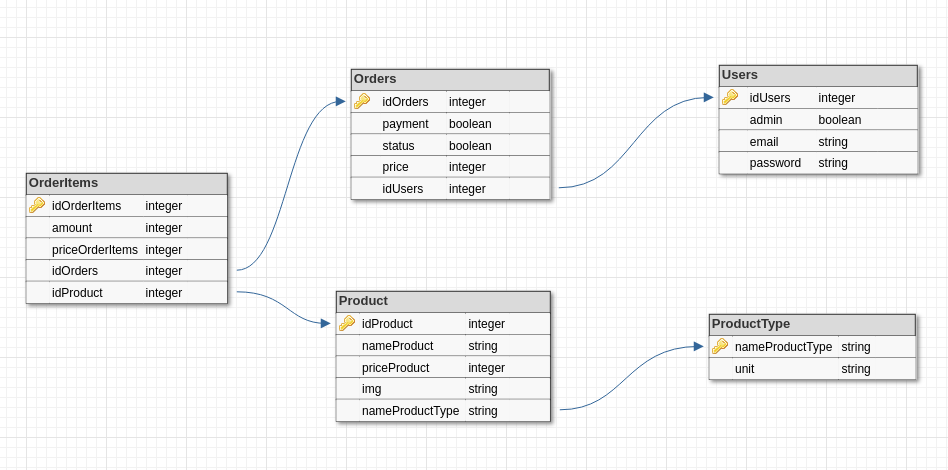
\includegraphics[width=\textwidth]{second_sprint/db_schema.png}
  \caption{\label{fig:schema} The database schema.}
\end{figure}

\begin{itemize}
  \item[\textbf{Users:}] Contains the Users, both admins and non-admins. The
    email is used to identify User at login, so no username is needed.
  \item[\textbf{Orders:}] Used to represent the shopping basket before an
    Order was made (\mintinline{python}{payment == False}) an Order that has
    been paid but not yet processed and shipped (\mintinline{python}{payment
    == True and status == False}), as well as finished Orders
    (\mintinline{python}{status == True}). Each Order has one User.
  \item[\textbf{OrderItems:}] The mapping between Orders and Products
    (Products were previously known as Items, that is why the name is still
    OrderItems, may be subject to change in a later release). Keeps track
    of how many of each product is included in the Order, as well as the
    price of the Product at the time it was paid.
  \item[\textbf{ProductType:}] The different possible types of a product. With
    each ProductType there is an associated unit in which a given amount
    of that ProductType is measured.
  \item[\textbf{Product:}] The merchandise, including name, price, image and
    ProductType.
\end{itemize}
